% Author: Rasmus Pank Roulund
\documentclass[tikz]{standalone}

%adapted from http://tex.stackexchange.com/questions/167483/spanning-a-cell-across-several-rows-in-tikz-matrix

\usetikzlibrary{calc,trees,positioning,arrows,chains,shapes.geometric,%
    decorations.pathreplacing,decorations.pathmorphing,shapes,%
    matrix,shapes.symbols,fit}

\pgfdeclarelayer{back}
\pgfsetlayers{back,main}

\tikzstyle{block} = [draw, fill=blue!20, rectangle, 
    minimum height=3em, minimum width=4em]

\tikzstyle{wblock} = [draw, rectangle, 
    minimum height=3em, minimum width=4em]


\begin{document}
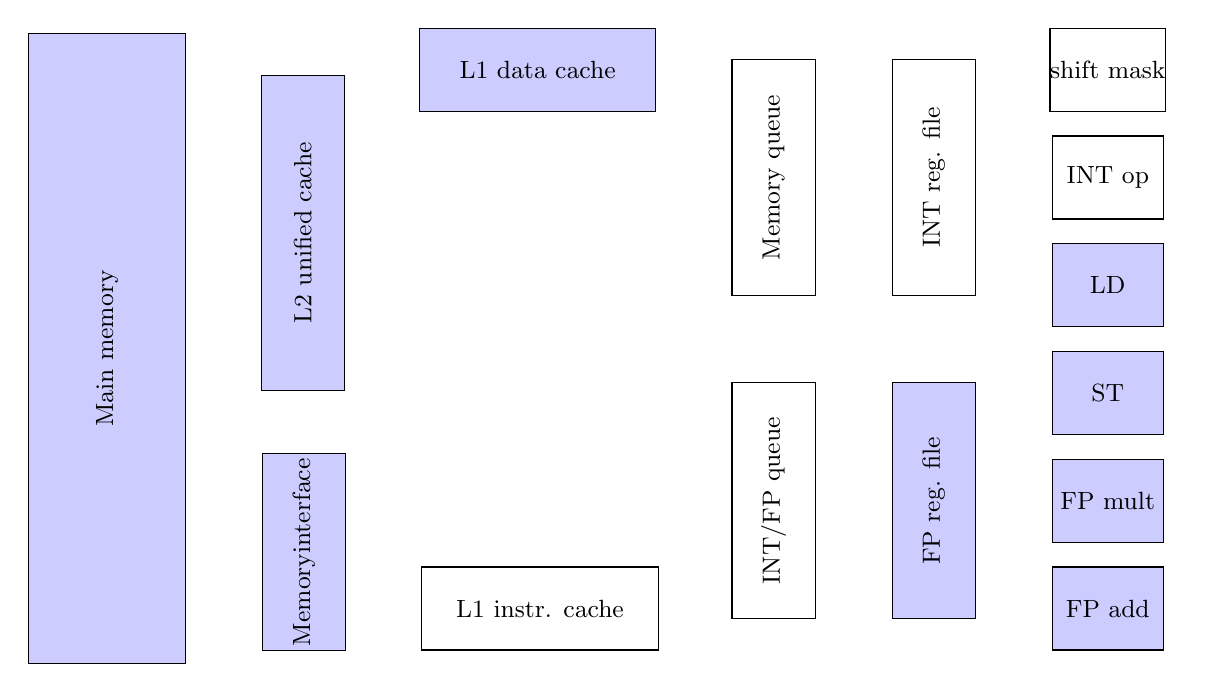
\begin{tikzpicture}[auto, node distance=2.5cm,>=latex',font=\small,
    every node/.style={inner sep=0pt,rectangle, minimum height=2.5em, text centered}]
    \matrix (m) [ampersand replacement=\&,column sep=1.5mm, row sep=3mm]
    {
      \node (sm) [wblock] {shift\newline{} mask}; \&
      \\
      \node (intop) [wblock] {INT\newline{} op}; \&
      \\
      \node (ld) [block] {LD}; \&
      \\
      \node (st) [block] {ST}; \&
      \\
      \node (fpmult) [block] {FP\newline{} mult}; \&
      \\
      \node (fpadd) [block] {FP\newline{} add}; \&
      \\
    };

\node (intregfile) [wblock,rotate=90,minimum width=3cm] at($(intop.west) - (1.5cm,0cm)$) {INT reg. file};
\node (fpregfile) [block,rotate=90,minimum width=3cm] at($(fpmult.west) - (1.5cm,0cm)$) {FP reg. file};

\node (memqueue) [wblock,rotate=90,minimum width=3cm] at($(intregfile.north) - (1.5cm,0cm)$) {Memory queue};
\node (intfpqueue) [wblock,rotate=90,minimum width=3cm] at($(fpregfile.north) - (1.5cm,0cm)$) {INT/FP queue};

\node (l1d) [block,minimum width=3cm] at($(sm.west) + (-6.5cm,0cm)$) {L1 data cache};
\node (l1i) [wblock,minimum width=3cm] at($(fpadd.west) + (-6.5cm,0cm)$) {L1 instr. cache};


\node (ram) [block,rotate=90,minimum width=8cm, minimum height=2cm] at($(fpadd.west) + (-12.cm,3.3cm)$) {Main memory};

\node (vRAM1) [coordinate] at($(ram.south east)!.4!(ram.south)$) {};
\node (vRAM2) [coordinate] at($(ram.south west)!.4!(ram.south)$) {};

\node (l2cache) [block,rotate=90,minimum width=4cm] at($(l1d.west)!.5!(vRAM1) + (0,-1.5cm)$) {L2 unified cache};
\node (memif) [block,rotate=90,minimum width=2.5cm] at($(l1i.north west)!.5!(vRAM2)$) {Memory\newline{}interface};

% \coordinate (aux1) at (D.west |- A.north);
% \coordinate (aux2) at ($(C.south west) - (3mm,0mm)$);
% \node[block, fit=(aux1)(aux2), inner sep=-.6pt] (X) {}; 
% \node[text width=3cm, text centered, anchor=center, rotate=90] at (X.center) {Main memory};


  \end{tikzpicture}
\end{document}
%%% Local Variables: 
%%% mode: latex
%%% TeX-master: t
%%% End: 
